\chapter{Project Risk Management}

Project Risk Management is defined by PMBoK as "the process of conducting risk management planning, identification, analysis, response planning and monitoring and control on a project" \parencite{pmbok}. The objectives of this project management area are to increase the probability and impacts of positive events, while at the same time decreases the same of negative events within the scope of the project. 

\section{Processes}

There are a number of processes involved in the Risk Management aspect of a project plan, illustrated in Figure~\ref{fig:risks}.

\begin{enumerate}
\item Plan Risk Management
\begin{itemize}
\item The process of "defining how to conduct risk management activities for a project" \parencite{pmbok}.
\end{itemize}
\item Identify Risks
\begin{itemize}
\item Determining "which risks may affect the project and documenting their characteristics" \parencite{pmbok}.
\end{itemize}
\item Perform Qualitative Risk Analysis
\begin{itemize}
\item This is the process of prioritising risks. These risks can then be sent "for further analysis or action by assessing and combining their probability of occurrence and impact" \parencite{pmbok}.
\end{itemize}
\item Perform Quantitative Risk Analysis
\begin{itemize}
\item This is the process of "numerically analysing the effect of identified risks on the overall project objectives" \parencite{pmbok}.
\end{itemize}
\item Plan Risk Responses
\begin{itemize}
\item This builds on the results of the previous processes. This process plans for how each risk should be managed, and which person is responsible for the management of that particular risk.
\end{itemize}
\item Control Risks
\begin{itemize}
\item This is the process of "implementing the risk response plans, tracking identified risks, identifying new risks, and evaluating risk process effectiveness throughout the project" \parencite{pmbok}.
\end{itemize}
\end{enumerate}
\begin{figure}[H]
\caption{Risk Management Processes}
\label{fig:risks}
\end{figure}

One of the main risks in a software project is the choice of the architecture. A qualified software architect, with the experience necessary to properly evaluate and choose a software solution, would play a major role in negating this risk. The choice of a proper architecture lays the groundwork for the future development, and is a mistake that is very hard to rectify further on in the project lifecycle.

\section{Techniques}

\section{Risk Management Plans}

The main risks exposed by this project are design choices and requirements elicitation. A big risk in the project would be a choice to develop a more generic solution, and tailor it towards the client, rather than develop specifically for the client. This approach would cost more over the lifetime of the project, but it would also allow the project to reach a larger potential customer base. The design of the system as a more modular, separate unit, composed of many parts, would increase development time and complexity, but long term, it would allow for reduced costs with regards towards the various kinds of maintenance: corrective, adaptive and perfective. 

\begin{enumerate}
\item Use of Commercial Off The Shelf (COTS) software within the application
\begin{itemize}
\item Is there a cost to the user to get this software? What happens if it's updated/discontinued?
\end{itemize}
\item Staff Experience with Frameworks
\begin{itemize}
\item Are the staff experienced with the chosen frameworks? Will it affect development?
\end{itemize}
\item Choice of frameworks
\begin{itemize}
\item Risks associated with choosing more modern frameworks over those that developers have experience with, for reasons such as extensibility, performance (e.g. Spring MVC Vs Enterprise Java Beans; Tomcat 7 Vs Glassfish).
\end{itemize}
\item Changes to project modules
\begin{itemize}
\item What modules would require the most work to change? How much work? How will it affect other modules?
\end{itemize}
\end{enumerate}

\begin{figure} [H]
\begin{center}
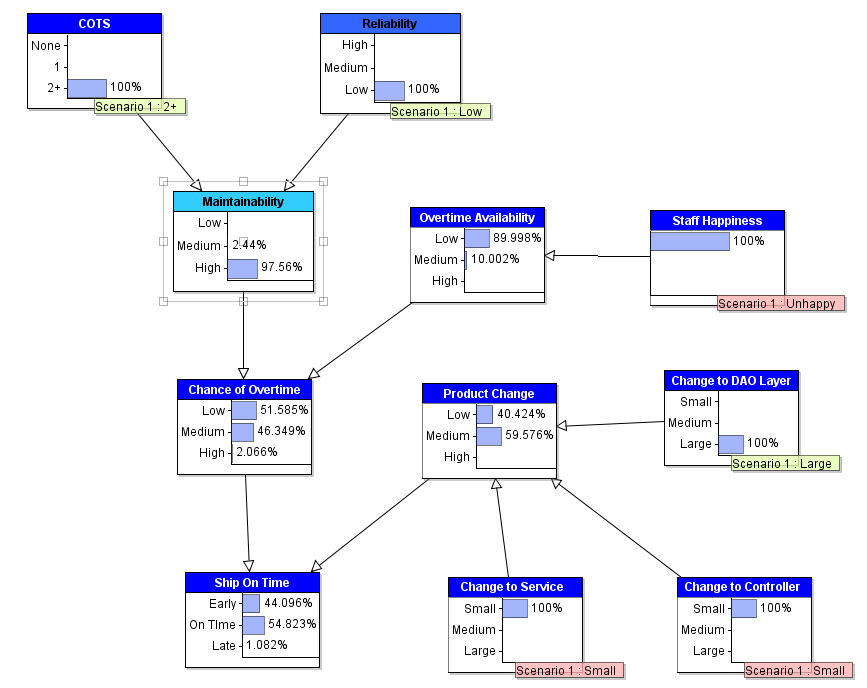
\includegraphics[scale=0.7]{risk.png}
\caption{Agena Risk Model}
\label{fig:agenarisk}
\end{center}
\end{figure}